% Desarrollo
\chapter{Desarrollo} \label{ch:des}
En este capítulo se detalla el desarrollo del proyecto siguiendo las etapas de diseño descritas. Se comenzará por la preparación del entorno y posteriormente se describirá la implementación de los escenarios en GCP.

\section{Preparación del entorno} \label{sec:prep}
  Antes de comenzar, es necesario disponer de una cuenta en Google Cloud Platform, así como disponer de un proyecto creado. Para crear un proyecto, basta con seleccionar o crear uno en la página del selector de proyectos de Google Cloud. 

  \begin{figure}[h]
  \centering
  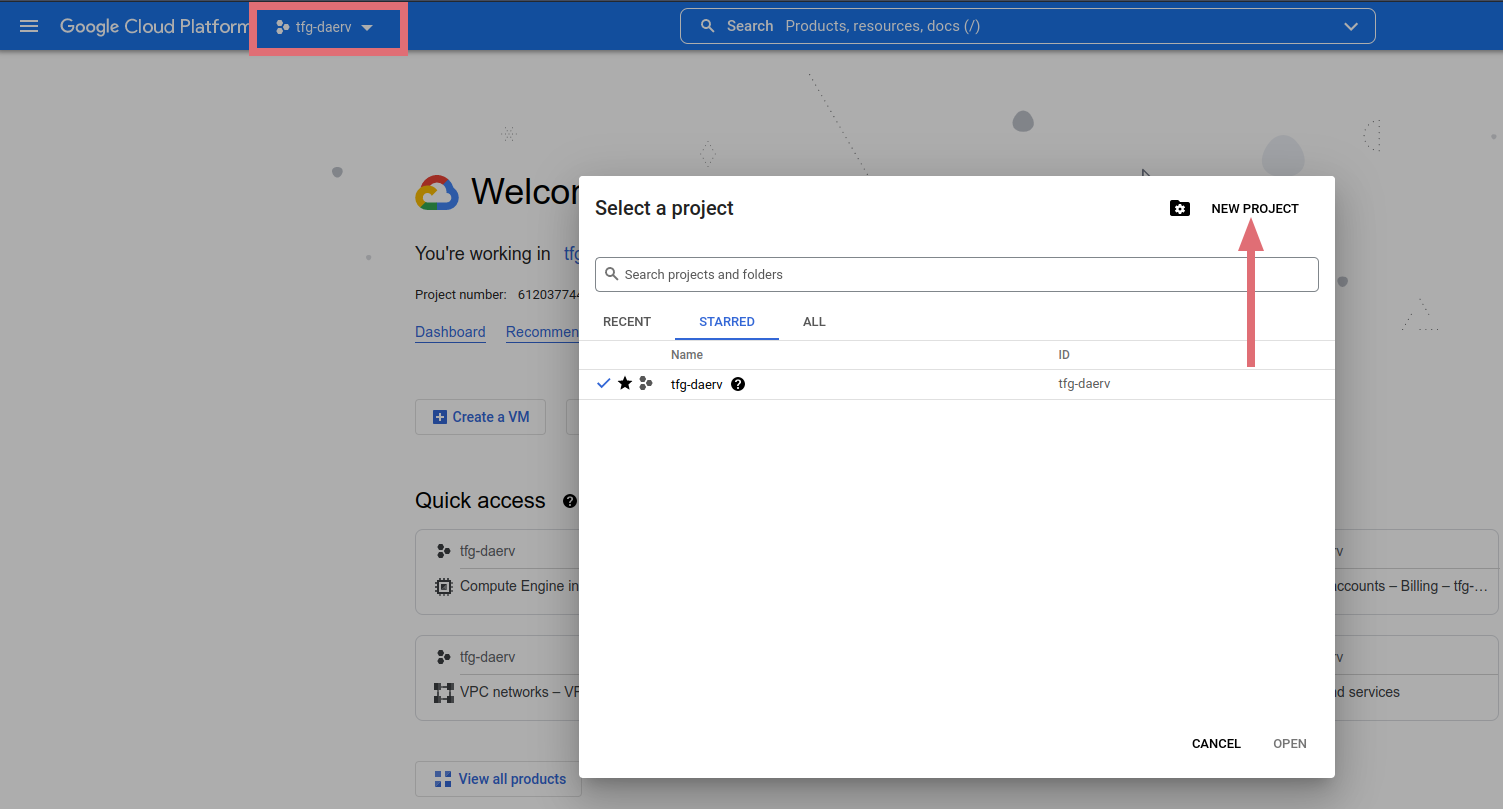
\includegraphics[width=\textwidth]{../imgs/desarrollo/entorno/project.png}
  \caption{Selección de un proyecto en Google Cloud}
  \label{fig:ent1}
  \end{figure}

  Una vez tengamos creada una cuenta y un proyecto en ella, debemos habilitar la API de Google Compute Engine~\cite{des1} para nuestro proyecto en la consola de GCP. También es necesario instalar tanto Terraform como la CLI de Google Cloud. Una vez hecho todo esto, lo primero es autenticarse con GCP. Para ello, basta con ejecutar \texttt{gcloud auth application-default login} en la terminal. Esto nos dirigirá a una página donde podremos iniciar sesión con nuestra cuenta de Google para permitir el acceso a nuestros datos de GCP.

  Para poder realizar peticiones desde Terraform a la API de GCP, también es necesario autenticarse para así probar que somos quien están realizando esas peticiones. Hay varias formas de realizar esta autenticación. Una de ellas es mediante las Cuentas de Servicio de Google Cloud, para la cual hay que seguir los siguientes pasos:

  \begin{enumerate}
    \item En el apartado de Cuentas de Servicio de la consola de Google Cloud debemos elegir una cuenta existente, o crear una nueva. A la hora de crearla hay que tener en cuenta que es necesario asignar permisos de edición.
    \item En la sección de claves, debemos generar una clave y descargarla en formato JSON, ponerle un nombre del que nos vayamos a acordar y almacenarla en un lugar seguro. 
    \item Para proporcionarle la clave descargada a Terraform, lo haremos mediante la variable de entorno \texttt{GOOGLE\_APPLICATION\_CREDENTIALS}, asignándole como valor el de la ruta al archivo con la clave ejecutando el siguiente comando:

      \begin{lstlisting}[language=Bash]
	export GOOGLE\_APPLICATION\_CREDENTIALS=\{\{path\}\}\end{lstlisting}

      Para que las credenciales se guarden entre sesiones, es necesario añadir esta línea a un fichero de inicio como \texttt{bash\_profile} o \texttt{bashrc}. Una opción alternativa a la variable de entorno sería proporcionar a Terraform el path a la clave en la configuración del provider, dentro del fichero \texttt{main.tf}.
  \end{enumerate}

  Por último, en el fichero \texttt{.tf} que va a contener todo el código necesario para alcanzar el estado necesario de nuestra infrestructura, hay que configurar el provider de Google. Para ello, en dicho fichero, que normalmente se llama \texttt{main.tf} añadiríamos el código mostrado en la parte inferior, y ejecutaríamos la instrucción \texttt{terraform init} en el mismo directorio donde se encuentra el fichero para que todos e configure correctamente. 

  \begin{lstlisting}[language=Bash]
  provider "google" {
    project = var.project_id
    region  = var.region
    zone    = var.zone
  }\end{lstlisting}

  En este caso, se han utilizado variables almacenadas en el fichero \texttt{variables.tf} para asignar el valor a los parámetros. Además, también cabe mencionar que por comodidad se ha empleado la misma región y zona en todos los escenarios desplegados, ya que el valor de este campo simplemente determina el centro de datos de Google en el que se despliegua la infraestructura.

  Una vez hechas estas configuraciones, ya podemos desarrollar nuestro código Terraform y ordenar que se despliegue la infraestructura en nuestro proyecto simplemente con el comando \texttt{terraform apply}, destruir la infrestructura desplegada con \texttt{terraform destroy} o consultar el estado de los recursos desplegados con la orden \texttt{terraform state list}, entre otras muchas opciones.


\clearpage 
\section{Escenarios de red} \label{sec:scen}
  En esta sección se van a presentar los escenarios de red a simular y se va a desarrollar su implementación en Google Cloud. 

\subsection{Smart Office 1} \label{sec:so1}
\subsubsection{Descripción}
  El escenario \textit{Smart Office 1} simula una oficina que cuenta con una red LAN cableada Ethernet en la que se encuentran conectados los sistemas de la oficina. En dicha oficina, existe un sistema de impresión que permite a los empleados realizar impresiones desde sus ordenadores. Dicho sistema cuenta con uno o varios dispositivos basados en Linux, de los cuales uno es una impresora conectada a un servidor remoto propio de la marca en un entorno Cloud.

  El atacante se encuentra conectado a una red local inalámbrica en la que que también se encuentra el PC de un empleado de la empresa. Dicho empleado está a su vez conectado a la red interna de la empresa mediante una red cableada Ethernet. El objetivo del atacante es lanzar un ataque sobre el servicio de impresión en el que, mediante la modificación del firmware, logre acceder a la red local remota. La impresora no requiere autenticación antes de la actualización de firmware, por tanto esta sería la vulnerabilidad a aprovechar por el atacante.

  \begin{figure}[h]
  \centering
  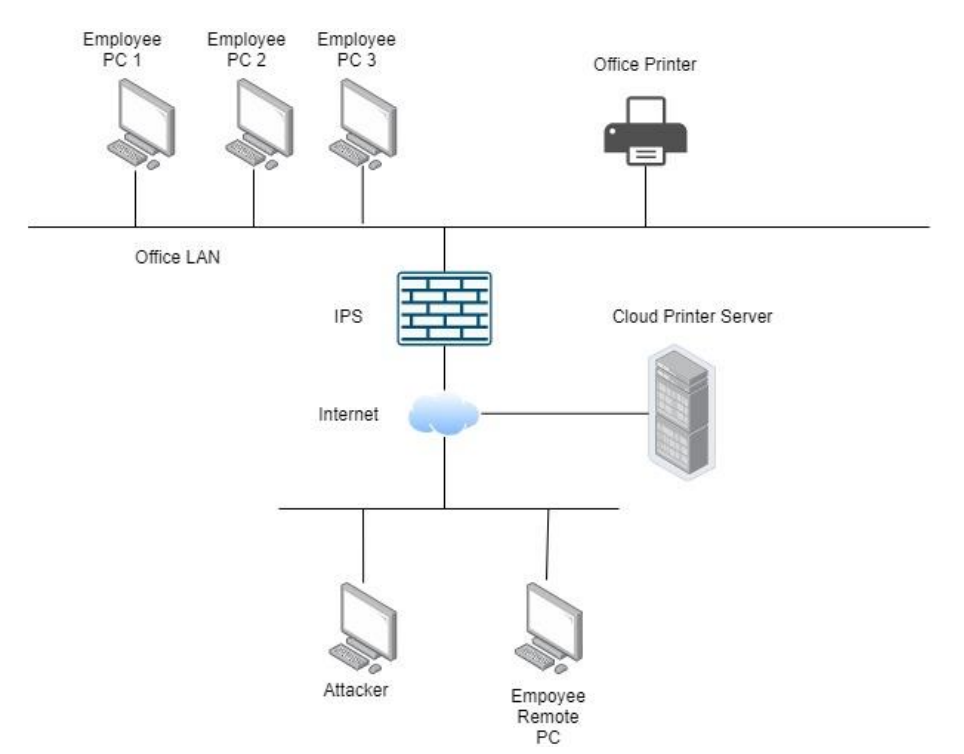
\includegraphics[width=0.7\textwidth]{../imgs/desarrollo/escenarios-de-red/smart-office-1/smart-office-1.png}
  \caption{Topología del escenario Smart Office 1}
  \label{fig:so1-t}
  \end{figure}

  El atacante deberá ganar acceso al equipo del empleado remoto, que es quien tiene conexión con la red interna de la empresa, mediante la explotación de alguno de sus servicios. Una vez hecho esto, recopilaría información referente a la impresora y solicitaría el procesamiento de un documento malicioso, cuyo contenido será enviado y embebido mediante comandos PJL (\textit{Printer Job Languaje}). La aleatoriedad de los comandos haría imposible su detección por parte de los sistemas de seguridad de la empresa, de forma una vez lleguen a la impresora víctima, esta reconocerá que el trabajo de impresión contiene una actualización de firmware válida y permitirá al atacante realizar modificaciones arbitrarias en el área de almacenamiento del firmware. En esta situación, el atacante podrá acceder al servidor de impresión, que actúa como un log descentralizado y podría contener información sensible sobre lo que haya impreso cada empleado.

\subsubsection{Implementación}
  Para la implementación de este escenario se han definido 3 VPCs. Una de ellas representa la oficina interna, donde se ubican 2 instancias de Compute Engine basadas en Linux que representan equipos de empleado y la impresora. Esta red interna está segmentada, es decir, los equipos de empleado se ubican en una LAN diferente a la impresora, siendo una LAN una subred de la VPC. Otra VPC simula la red externa de la empresa, donde se localizan el equipo del atacante y el empleado remoto, ambos en la misma LAN y también basados en Linux. Finalmente, en la tercera VPC se aloja el servidor de impresión.


  \begin{table}[h]
    \begin{center}
      \begin{tabular}{ | m{5cm} | w{c}{3cm} | w{c}{2,5cm} | m{3,75cm} | }
        \hline\rowcolor{oranget} \centering\textbf{VPC} & \textbf{LAN} & \textbf{Rango IP} & \textbf{Equipos} \\ \hline
        \multirow{2}{*}{office-internal-network} & employees-lan & 10.10.10.0/24 & employee-pc-1 employee-pc-2 \\ \cline{2-4}
         & printer-lan & 10.10.20.0/24 & printer \\ \hline\rowcolor{oranger} 
        internal-server-network & printer-server-lan & 10.10.30.0/24 & cloud-printer-server \\ \hline
        office-external-network & office-external-lan & 10.10.40.0/24 & employee-remote-pc attacker \\ \hline
      \end{tabular}
      \caption{Estructura del escenario Smart Office 1}
      \label{tab:vpc1}
    \end{center}
  \end{table}


  La conectividad entre las VPCs es la siguiente: se ha establecido un VPC Peering entre las redes externa e interna de la oficina, de forma que se permite la conectividad entre las direcciones IP internas de ambas, lo que simularía la conexión cableada Ethernet previamente mencionada. A su vez, también existe un VPC Peering entre la red interna de la oficina y la red donde se ubica el servidor de impresión, que no es accesible desde internet. De esta forma, los equipos de la red interna de la oficina tendrán conectividad tanto con la red externa como con la red del servidor, mientras entre la red externa y el servidor no existe dicha conectividad.

  En cuanto al acceso a Internet, en cada una de las redes de la oficina se ha desplegado un Cloud Router con su respectivo Cloud NAT, lo que permite que las instancias sin direcciones IP externas que se encuentran en ambas redes puedan crear conexiones salientes a Internet. El servidor es local y por tanto no se ha configurado su acceso a internet. 

  Tal y como se mencionó en el estado del arte, que las instancias tengan conectividad no quiere decir que esta sea efectiva, ya que una de las reglas de FW implícitas rechaza todo el tráfico entrante. Es decir, para que sea posible el intercambio de tráfico deseado, no basta con hacer un peering entre las VPC, sino que hay que definir reglas de FW que permitan o restrinjan el tráfico que se intercambia. Para replicar este escenario, ha sido necesario crear las siguientes:

  \begin{table}[h]
    \begin{center}
      \footnotesize\hspace*{-1.75cm}\begin{tabular}{ | m{2cm} | m{2cm} | w{c}{1,5cm} | m{2cm} | m{2cm} | m{2cm} | w{c}{1,25cm} | w{c}{1,25cm} | }
        \hline\rowcolor{oranget} \centering\textbf{Nombre} & \centering\textbf{VPC} & \textbf{Dirección} & \centering\textbf{Origen} & \centering\textbf{Destino} & \centering\textbf{Protocolos} & \textbf{Puertos} & \textbf{Acción} \\ \hline
        allow-internal & office-internal-network & INGRESS & 10.10.10.0/24 10.10.20.0/24 & \centering- & TCP, UDP, ICMP & 0-65535 & ALLOW  \\ \hline\rowcolor{oranger}
        allow-external & office-external-network & INGRESS & 10.10.40.0/24 & \centering- & TCP, UDP, ICMP & 0-65535 & ALLOW  \\ \hline
        allow-internal-from-external & office-internal-network & INGRESS & employee-remote-pc (IP) & \centering- & TCP, UDP, ICMP & 0-65535 & ALLOW  \\ \hline\rowcolor{oranger}
        allow-external-from-internal & office-external-network & INGRESS & 10.10.10.0/24 10.10.20.0/24 & employee-remote-pc (IP) & TCP, UDP, ICMP & 0-65535 & ALLOW  \\ \hline
        allow-printer-from-server & office-internal-network & INGRESS & 10.10.30.0/24 & printer (IP) & TCP, UDP, ICMP & 0-65535 & ALLOW  \\ \hline\rowcolor{oranger}
        allow-server-from-printer & internal-server-network & INGRESS & printer (IP) & 10.10.30.0/24 & TCP, UDP, ICMP & 0-65535 & ALLOW  \\ \hline 
      \end{tabular}\hspace*{-1.75cm}
      \caption{Reglas de FW del escenario Smart Office 1}
      \label{tab:fw1}
    \end{center}
  \end{table}

  \textbf{allow-internal:} esta regla se aplica a la VPC de la red interna de la oficina. Permite la entrada de tráfico de cualquier protocolo por cualquier puerto siempre y cuando la dirección IP origen se encuentre dentro de la red interna. Al no especificarse destino, aplica a toda la VPC, por lo que en resumen esta regla permite que las instancias de la red interna de la oficina intercambien tráfico entre sí.

  \textbf{allow-external:} análogamente a allow-internal, esta regla permite que el atacante y el empleado remoto intercambien tráfico entre sí, al encontrarse en la misma LAN.

  \textbf{allow-internal-from-external:} se aplica a la red interna de la oficina, de forma que permite la entrada del tráfico procedente únicamente del empleado remoto, ya que es quien está conectado mediante cable a la red interna. Al estar en VPCs distintas, se especifica como origen la IP del empleado remoto. 

  \textbf{allow-external-from-internal:} análogamente a la anterior, se aplica a la red externa de la oficina, y permite la entrada de tráfico procedente tanto de los empleados como de la impresora únicamente hacia empleado remoto, especificando su IP. 

  \textbf{allow-printer-from-server:} se aplica en la red interna de la oficina, permite el tráfico entrante procedente de la LAN donde se encuentra el servidor hacia la impresora.

  \textbf{allow-server-from-printer:} análogamente a la anterior, el servidor sólo acepta tráfico de entrada procedente de la impresora.

  Es necesario puntualizar algunos aspectos acerca de las reglas de FW comunes a todos los escenarios:

  \begin{itemize}
    \item Como se puede apreciar, muchas de las reglas están configuradas para permitir el tráfico de los protocolos TCP, UDP e ICMP por todos los puertos. Por supuesto esto no sería lo óptimo, y cuando se conociese con detalle los servicios y comunicaciones que realiza cada máquina, estas reglas se podrían modificar para  concretar mejor el tráfico que permiten. 

    \item Las reglas de la tabla tienen asignada una prioridad mayor que aquellas reglas que define Google Cloud por defecto. Por tanto, todo el tráfico de entrada a cualquiera de las VPCs que no aparezca definido en la tabla será rechazado. Además, en la tabla sólo se muestran las reglas custom que ha sido necesario crear, por lo que aunque no aparezca, es efectiva la regla por defecto de Google Cloud que permite el tráfico saliente desde cualquier instancia hacia cualquier destino usando cualquier protocolo por cualquier puerto.

    \item A la hora de especificar los orígenes y destinos en Terraform, se hace una referencia al objeto. Es decir, no se especifica como origen un string con el rango de IPs de una subred, si no que se hace referencia al rango de IP que tenga asignada la LAN en ese momento, de forma que si esas IP cambian, no es necesario cambiar la definición de la regla. Esto se puede ver con más detalle en el Anexo \ref{sec:anxE}.
  \end{itemize}

  En cuanto al aprovisionamiento, la idea en este escenario sería crear imágenes en Google Cloud a partir de una ISO ya existente, como por ejemplo una imagen basada en Kali Linux para el atacante, o imágenes Windows de usuario para los empleados, ya que las imágenes Windows disponibles en Google Cloud son de Windows Server. Estas imágenes personalizadas se almacenarían en Google Cloud y se podría pasar como parámetro a la instancia a la hora de construirla, como también se puede ver en el Anexo \ref{sec:anxA}.

  \clearpage
  \begin{figure}[h]
  \centering
  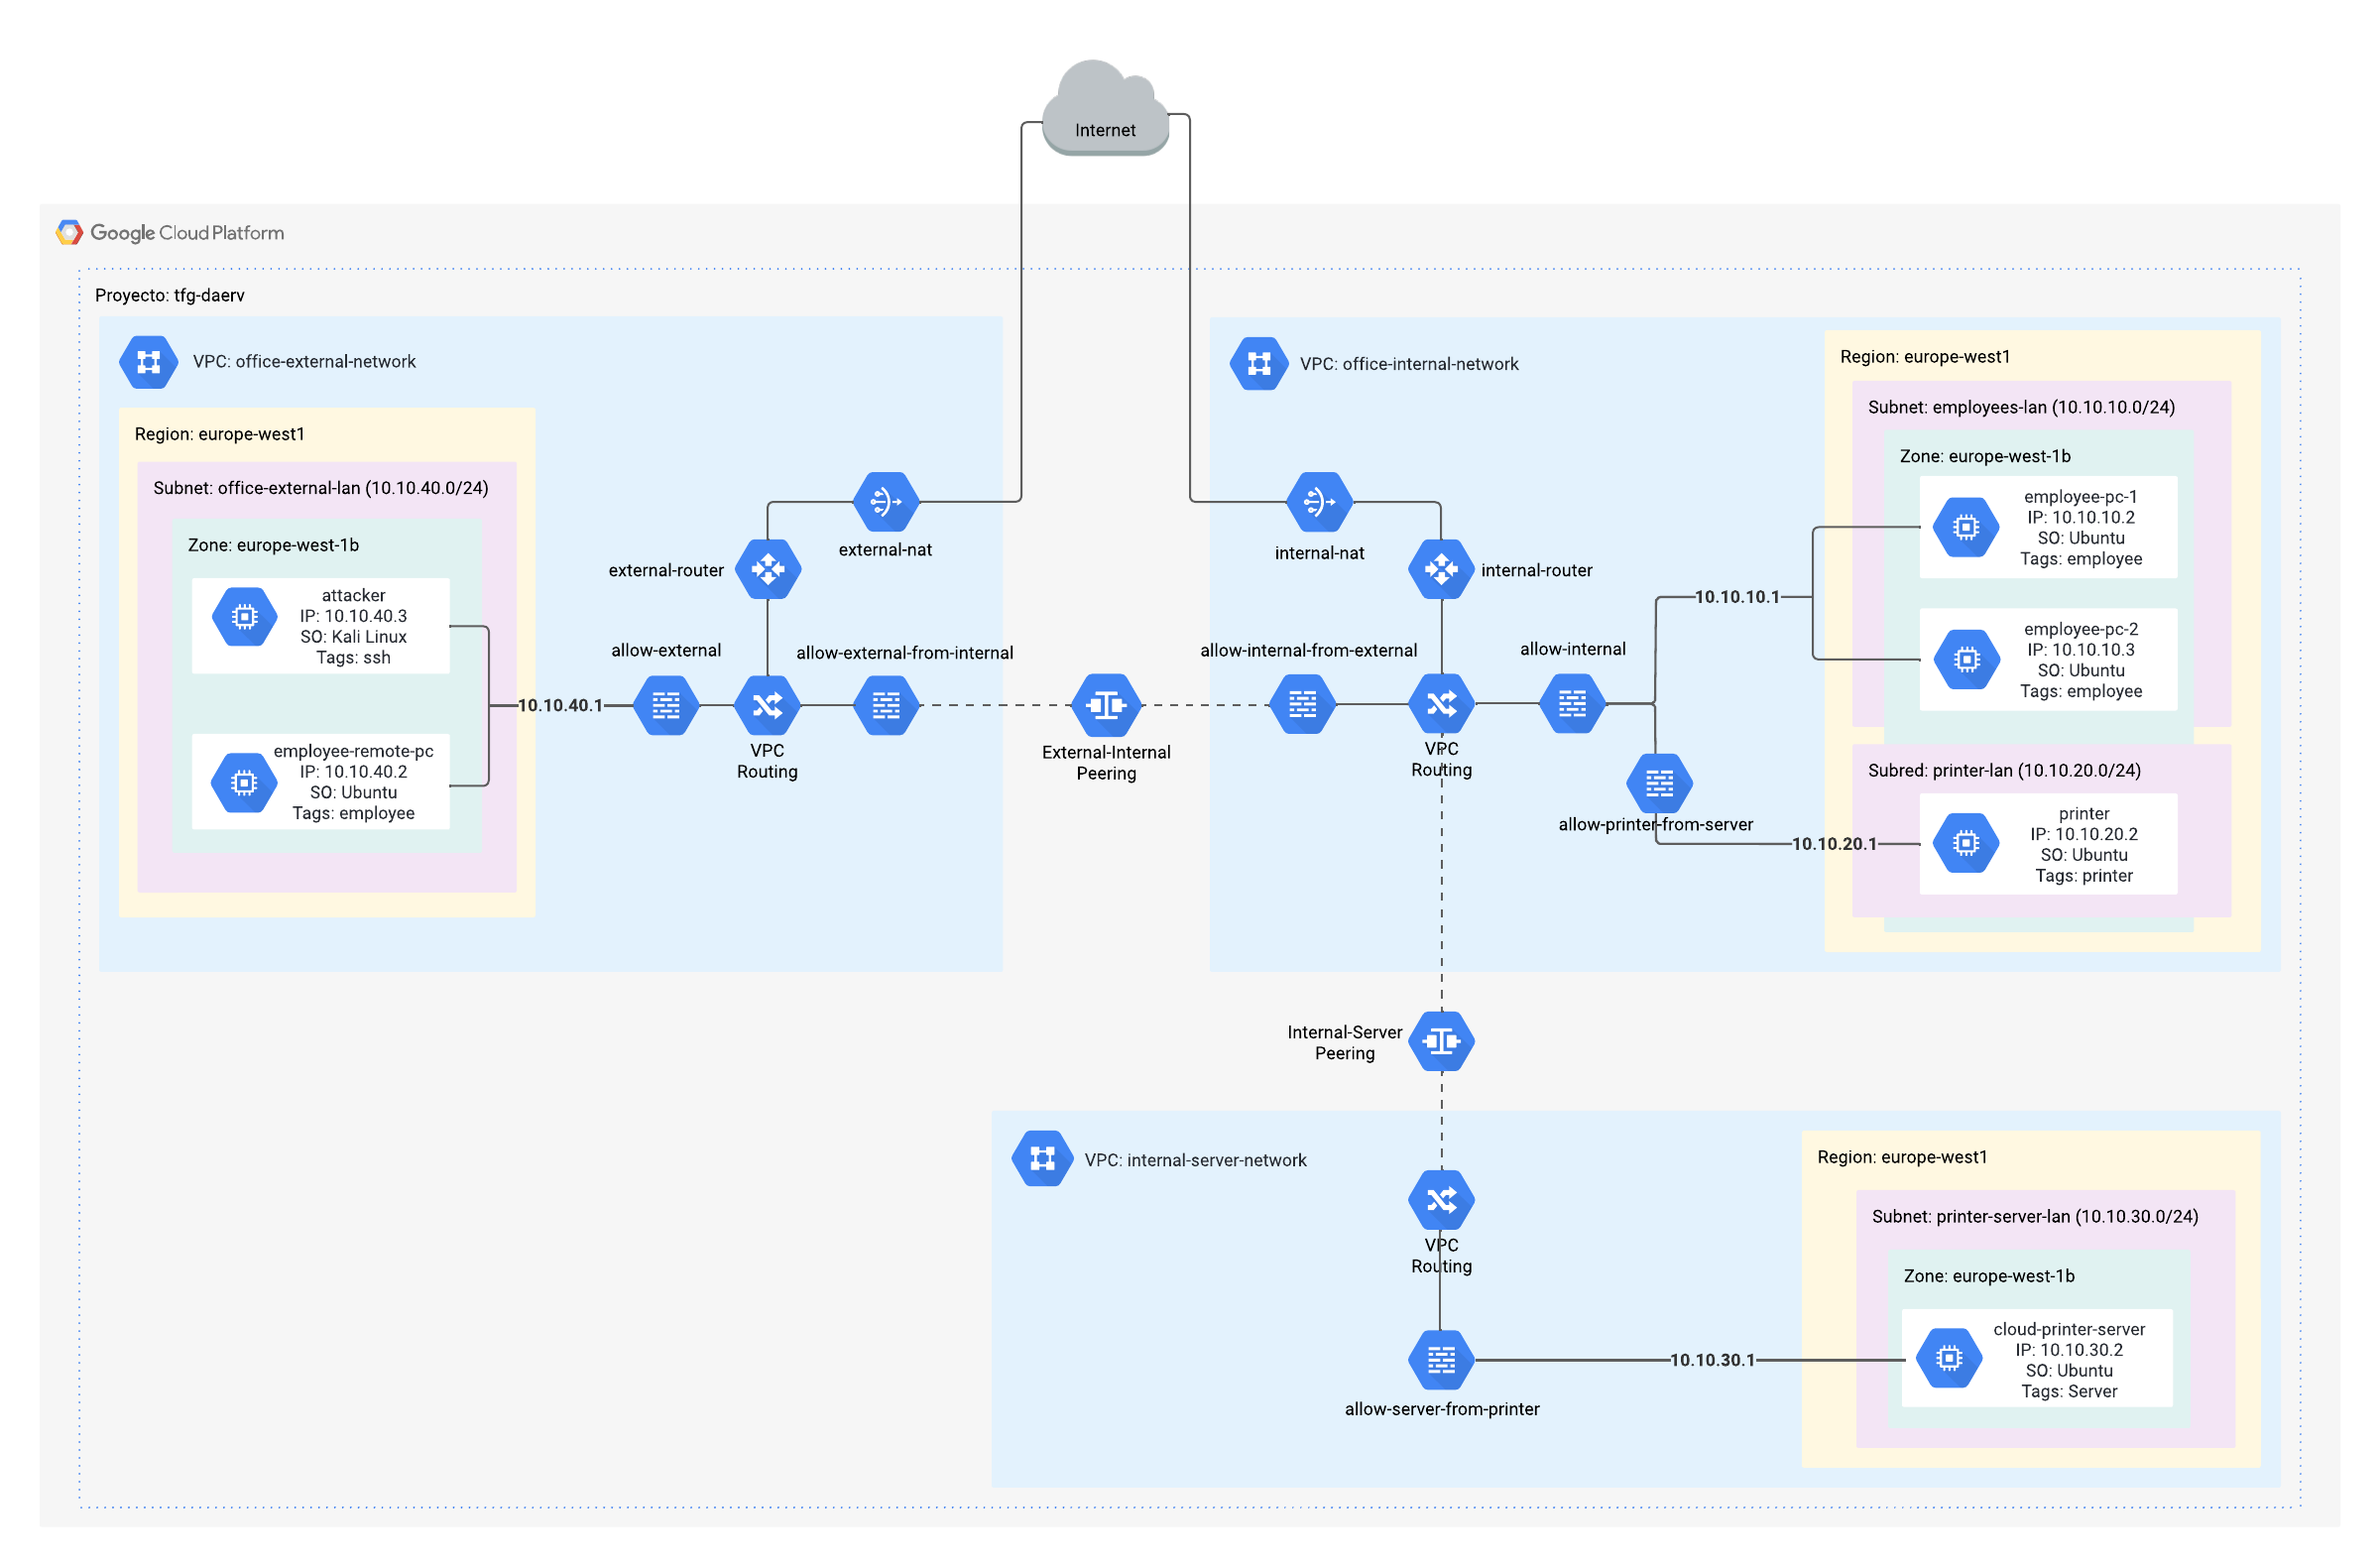
\includegraphics[width=1.45\textwidth, angle=270]{../imgs/desarrollo/escenarios-de-red/smart-office-1/EscenarioSmartOffice1V2.png}
  \caption{Implementación en GCP del escenario Smart Office 1}
  \label{fig:so1-i}
  \end{figure}
  \clearpage 

\subsection{Smart Office 2} \label{sec:so2}
\subsubsection{Descripción}
  El escenario \textit{Smart Office 2} plantea una oficina que cuenta con una red LAN cableada Ethernet en la que se encuentran conectados los sistemas de la oficina. En dicha LAN, existe un sistema de \textit{Smart Speaker} (micrófono y altavoz) que permite a los empleados hacer ciertas tareas utilizando órdenes de voz. Dicho sistema cuenta con uno o varios dispositivos basados en Linux que funcionan como clientes y que escuchan los comandos de voz en la oficina. Estos dispositivos se conectan a un hub interno que, mediante un protocolo IoT permite lanzar comandos básicos a los dispositivos (encendido, apagado, etc) y recibir mensajes de audio capturado a través de los micrófonos. Estos mensajes de audio se cifran y se envían de forma segura desde el hub a un servidor remoto localizado en un entorno Cloud.

  La empresa cuenta con un servicio VPN implementado en el router de entrada a la red LAN que permite a los empleados conectarse a dicha red de forma remota. Existe una vulnerabilidad en el cliente VPN de dicho servicio que permitiría a un atacante robar las credenciales del usuario a través de sus cookies y acceder a la red local. 

  
  El atacante se encuentra conectado a una red LAN en la que también se encuentra el PC de un empleado de la empresa. En dicho PC existe una vulnerabilidad en un servicio de escritorio remoto que permite al atacante acceder a las cookies almacenadas por el cliente VPN y robarlas para suplantar al empleado y acceder a la empresa a través del servicio VPN. Una vez en la red interna, el atacante es capaz de acceder al hub Linux, que se comunica de forma insegura con los dispositivos \textit{Smart Speaker}, siendo capaz de activarlos y desactivarlos arbitrariamente y de recuperar el audio recogido por ellos antes de que se envíe al servidor remoto sin conocimiento de los empleados en la oficina. \\ 

  \begin{figure}[h]
  \centering
  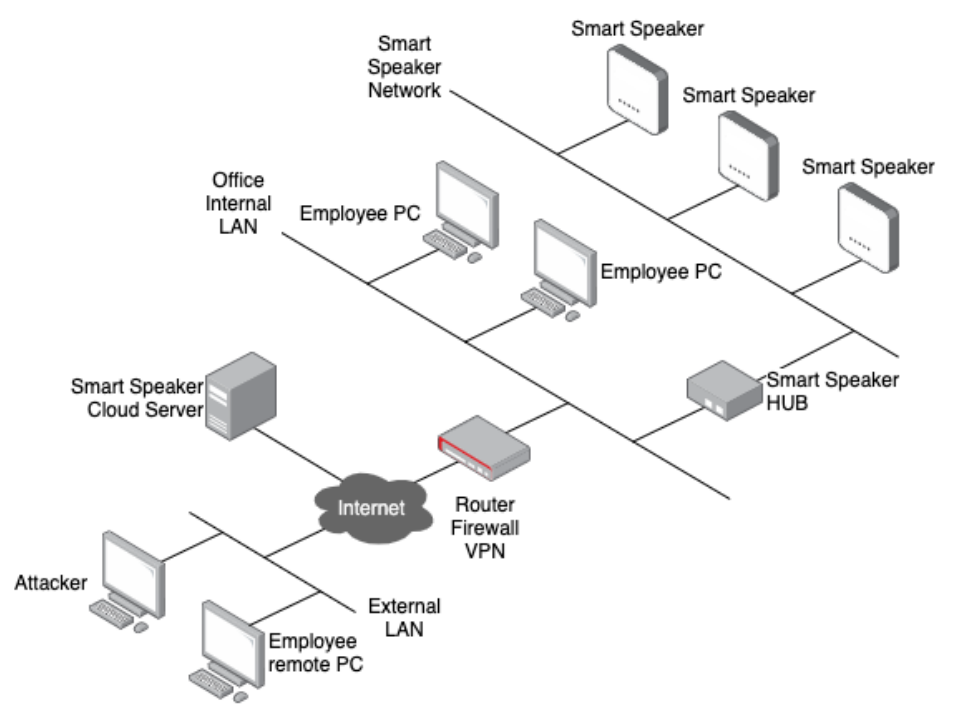
\includegraphics[width=0.7\textwidth]{../imgs/desarrollo/escenarios-de-red/smart-office-2/smart-office-2.png}
  \caption{Topología del escenario Smart Office 2}
  \label{fig:so2-t}
  \end{figure}

\subsubsection{Implementación}
  Este escenario se ha implementado siguiendo la misma base que en el escenario \textit{Smart Office 1}: una VPC una para cada red de oficina  y otra para la red del servidor. Al igual que en el caso anterior, en la red externa se ubica un PC de empleado y el equipo del atacante y en la red del servidor se encuentra el servidor cloud donde se envía el audio recogido por los altavoces inteligentes. La red interna está segmentada en dos LAN, una de ellas con dos PC de empleado y el hub, y la otra con los altavoces inteligentes. Todas los equipos son instancias de Google Compute Engine que usan imágenes Linux, aunque lo ideal sería, como ya se ha comentado, crear una imagen personalizada de Kali Linux para el atacante y una imagen de Windows de escritorio para los empleados. Las VM de la oficina tienen conexión a internet mediante sus respectivos Cloud Nat, mientras que el servidor no está expuesto.

   \begin{table}[h]
    \begin{center}
      \begin{tabular}{ | m{5cm} | w{c}{3cm} | w{c}{2,5cm} | m{3,75cm} | }
        \hline\rowcolor{oranget} \centering\textbf{VPC} & \textbf{LAN} & \textbf{Rango IP} & \textbf{Equipos} \\ \hline
        \multirow{2}{*}{office-internal-network} & office-internal-lan & 10.10.10.0/24 & employee-pc-1 employee-pc-2 smart-speaker-hub \\ \cline{2-4}
         & speakers-lan & 10.10.20.0/24 & smart-speaker-1 smart-speaker-2 smart-speaker-3 \\ \hline\rowcolor{oranger} 
        internal-server-network & speaker-server-lan & 10.10.30.0/24 & smart-speaker-cloud-server \\ \hline
        office-external-network & office-external-lan & 10.10.40.0/24 & employee-remote-pc attacker \\ \hline
      \end{tabular}
      \caption{Estructura del escenario Smart Office 2}
      \label{tab:vpc2}
    \end{center}
  \end{table}

  La interconexión entre las VPC difiere del escenario anterior. Entre la red interna de la oficina y la red del servidor, se mantiene el VPC peering que permite el intercambio de tráfico entre las VPC. En cambio, con el fin de simular la conexión VPN, entre las dos redes de oficina se ha empleado el servicio de Google Cloud llamado Cloud VPN. 

  Cloud VPN permite la conexión segura hacia la red de Google a través de un túnel VPN IPsec. Se ha creado una puerta de enlace VPN en cada una de las VPC, además de un túnel VPN que interconecta ambas puertas de enlace. Una puerta de enlace de VPN encripta el tráfico que viaja entre las dos redes a través de la Internet pública y la otra puerta de enlace de VPN lo desencripta. De esta forma, se protegen los datos mientras viajan por Internet. Cada puerta de enlace tiene una dirección IP pública. Google Cloud ofrece dos tipos de puertas de enlace de Cloud VPN: VPN con alta disponibilidad y VPN clásica. Se han empleado puertas de enlace de alta disponibilidad, dado que proporciona un 99.99\% de esta, además de un encaminamiento más eficiente.

  Pero no sólo ha bastado con crear las puertas de enlace y el túnel. Dado que no se ha entrado en la configuración de las instancias, no está implementado el cliente VPN que permite el intercambio de tráfico entre las puertas de enlace. Como solución temporal, para proporcionar conectividad entre las VPCs se han creado las siguientes rutas estáticas que permiten encaminar los paquetes entre los equipos de las redes de la oficina:

   \begin{table}[h]
    \begin{center}
      \begin{tabular}{ | m{3,5cm} | m{3cm} | w{c}{4cm} | m{3,75cm} | }
        \hline\rowcolor{oranget} \centering\textbf{Nombre} & \centering\textbf{Destino} & \textbf{VPC} & \textbf{Siguiente salto} \\ \hline 
        internal-vpn-route & 10.10.40.0/24 & office-internal-network & internal-vpn-tunnel \\ \hline\rowcolor{oranger}
        external-vpn-route & 10.10.10.0/24 10.10.20.0/24 & office-external-network & external-vpn-tunnel \\ \hline
      \end{tabular}
      \caption{Rutas del escenario Smart Office 2}
      \label{tab:rut2}
    \end{center}
  \end{table}

  Una vez existe la conectividad deseada entre los equipos, es necesario aceptar o denegar el tráfico entrante o saliente. Las reglas de firewall creadas se recogen a continuación:

  \begin{table}[h]
    \begin{center}
      \footnotesize\hspace*{-1.75cm}\begin{tabular}{ | m{2cm} | m{2cm} | w{c}{1,5cm} | m{2cm} | m{2cm} | m{2cm} | w{c}{1,25cm} | w{c}{1,25cm} | }
        \hline\rowcolor{oranget} \centering\textbf{Nombre} & \centering\textbf{VPC} & \textbf{Dirección} & \centering\textbf{Origen} & \centering\textbf{Destino} & \centering\textbf{Protocolos} & \textbf{Puertos} & \textbf{Acción} \\ \hline
        allow-internal & office-internal-network & INGRESS & 10.10.10.0/24 & \centering- & TCP, UDP, ICMP & 0-65535 & ALLOW  \\ \hline\rowcolor{oranger}
        allow-external & office-external-network & INGRESS & 10.10.40.0/24 & \centering- & TCP, UDP, ICMP & 0-65535 & ALLOW  \\ \hline
        allow-hub-from-speakers & office-internal-network & INGRESS & speaker (tag) & speaker-hub (tag) & TCP, UDP, ICMP & 0-65535 & ALLOW  \\ \hline\rowcolor{oranger}
        allow-speakers-from-hub & office-internal-network & INGRESS & speaker-hub (tag) & speaker (tag) & TCP, UDP, ICMP & 0-65535 & ALLOW  \\ \hline
        allow-internal-from-external & office-internal-network & INGRESS & employee-remote-pc (IP) & \centering- & TCP, UDP, ICMP & 0-65535 & ALLOW  \\ \hline\rowcolor{oranger}
        allow-external-from-internal & office-external-network & INGRESS & 10.10.10.0/24 & employee-remote-pc (IP) & TCP, UDP, ICMP & 0-65535 & ALLOW  \\ \hline
        allow-hub-from-server & office-internal-network & INGRESS & 10.10.30.0/24 & smart-speaker-hub (IP) & TCP, UDP, ICMP & 0-65535 & ALLOW  \\ \hline\rowcolor{oranger}
        allow-server-from-hub & internal-server-network & INGRESS & smart-speaker-hub (IP) & 10.10.30.0/24 & TCP, UDP, ICMP & 0-65535 & ALLOW  \\ \hline 
      \end{tabular}\hspace*{-1.75cm}
      \caption{Reglas de FW del escenario Smart Office 2}
      \label{tab:fw2}
    \end{center}
  \end{table}

  Se aprecia que las reglas de FW son prácticamente iguales a las del escenario Smart Office 1. La diferencia principal radica en que en este escenario, la regla allow-internal tiene como origen sólo el rango 10.10.10.0/24, lo que permite el intercambio de tráfico únicamente entre los ordenadores de empleado y el hub. Esto se debe a que la conexión con los altavoces está restringida, de forma que sea sólo el hub quien pueda recibir y enviar tráfico desde y hacia los altavoces, de ahí la necesidad de las reglas allow-speakers-from-hub y allow-hub-from-speakers, que limitan dicho tráfico haciendo uso de las etiquetas de red de cada instancia (recordemos que, al encontrarse en la misma VPC, es más cómodo usar los tags que las direcciones IP). Por la misma razón, la regla allow-external-from-internal también admite como IP origen únicamente la de la LAN interna, puesto que al empleado externo tampoco le está permitida la conexión directa con los altavoces.

  \clearpage
  \begin{figure}[h]
  \centering
  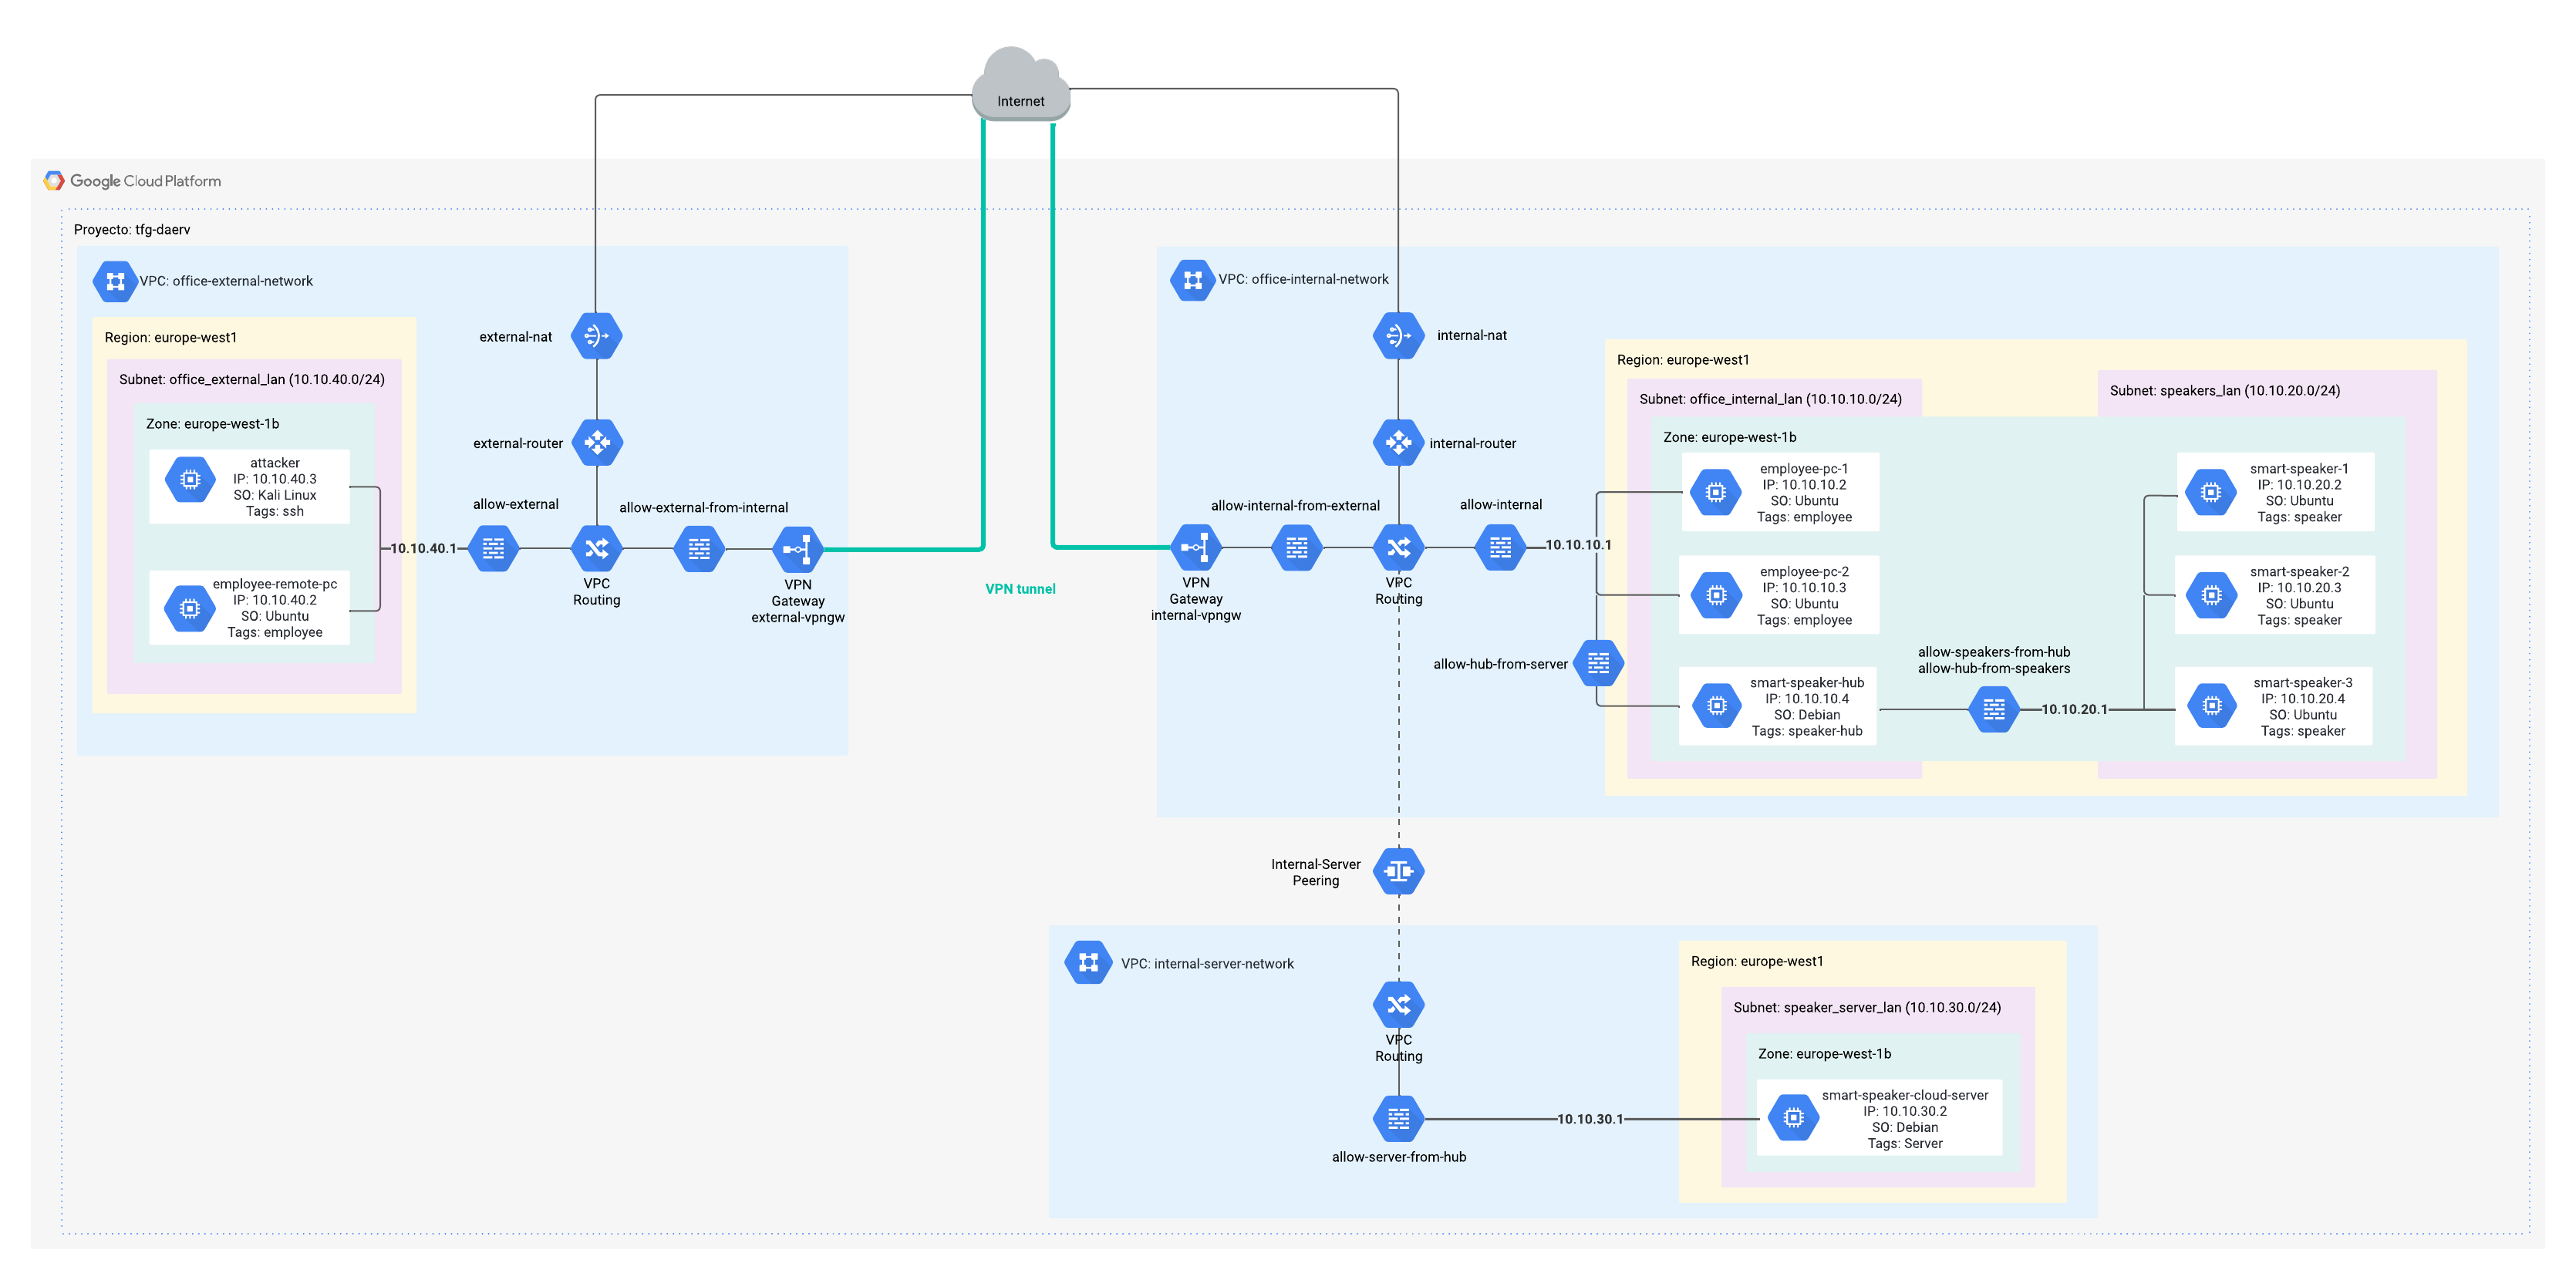
\includegraphics[width=1.45\textwidth, angle=270]{../imgs/desarrollo/escenarios-de-red/smart-office-2/EscenarioSmartOffice2V2.png}
  \caption{Implementación en GCP del escenario Smart Office 2}
  \label{fig:so2-i}
  \end{figure}
  \clearpage

\subsection{Smart Home} \label{sec:sh}
\subsubsection{Descripción}
  Este escenario representa una red de tipología \textit{Smart Home}, con un Access Point (AP) inalámbrico que ofrece conectividad a los dispositivos IoT de la casa. Además, la casa inteligente está controlada por un \textit{Homematic Central Control Unit} (CCU2) que expone la vulnerabilidad CVE-2019-14423 en un addon del firmware, lo que permite la ejecución remota de código (RCE) de forma que atacantes remotos autentificados podrían ejecutar comandos del sistema como root de forma remota a través de una simple petición HTTP.

  Además, otros dos dispositivos de la red exponen vulnerabilidades. En concreto, una bombilla inteligente (Signify Phillips Taolight Smart Wi-Fi Wiz Connected LED Bulb) permite a los usuarios remotos controlar su funcionamiento (CVE-2019-18980) y una cámara IP (Cisco Video Surveillance 8000 Series IP Cameras) podría permitir a un atacante adyacente no autenticado hacer que una cámara IP afectada se recargue (CVE-2021-1131). 

  El atacante tiene acceso a la red y puede explotar cualquiera de las tres vulnerabilidades mencionadas, que se explican con mayor detalle a continuación:

  La versión de firmware 2.31.25 del Homematic CCU2 muestra graves fallos de seguridad que permiten a un atacante obtener acceso completo al sistema y potencialmente también a los dispositivos periféricos conectados a través de comandos de shell que utilizan indebidamente la vulnerabilidad RCE. En cuanto a la bombilla, el modelo mencionado hace uso de una API no protegida (no hay autenticación ni cifrado para utilizarla) que permite que cualquiera pueda encenderla, apagarla o cambiar su brillo de forma remota. El único requisito es que el atacante tenga acceso a la red de la bombilla. Finalmente, en las cámaras IP de la serie 8000 de Cisco Video Surveillance, una vulnerabilidad en la implementación del protocolo Cisco Discovery permite que, enviando un paquete malicioso de Cisco Discovery Protocol a una cámara afectada, el atacante pueda realizar un ataque DoS al provocar que la cámara se recargue inesperadamente. 

  \begin{figure}[h]
  \centering
  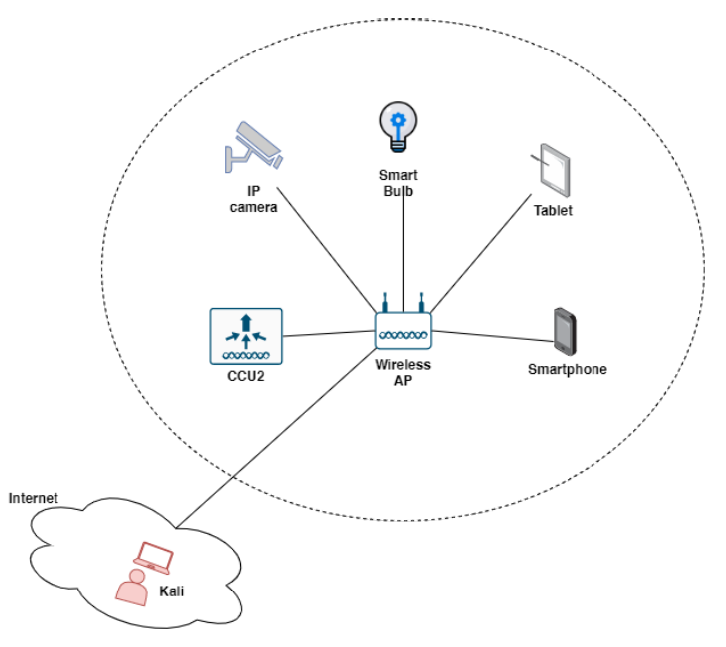
\includegraphics[width=0.5\textwidth]{../imgs/desarrollo/escenarios-de-red/smart-home/smart-home.png}
  \caption{Topología del escenario Smart Home}
  \label{fig:sh-t}
  \end{figure}

\subsubsection{Implementación}
  Para la simulación del escenario \textit{Smart Home} se han desplegado dos VPCs. La primera VPC representa la red local de la casa, que contiene 6 instancias Linux, que se corresponden con los dispositivos conectados a ella. La segunda VPC contiene únicamente el equipo del atacante, y su única función es la de brindarle a este acceso a la red de la casa, para lo cual se ha establecido un VPC peering entre ambas VPC. De esta forma, el atacante tiene acceso a la red local de la casa, lo que le permitirá explotar las vulnerabilidades que se han presentado anteriormente.

  \begin{table}[h]
    \begin{center}
      \begin{tabular}{ | m{5cm} | w{c}{2cm} | w{c}{2,5cm} | m{4,75cm} | }
        \hline\rowcolor{oranget} \centering\textbf{VPC} & \textbf{LAN} & \textbf{Rango IP} & \textbf{Equipos} \\ \hline
        smart-home & home-lan & 10.10.10.0/24 & wireless-ap, tablet, ccu2, ip-camera, smart-bulb, smartphone \\ \hline\rowcolor{oranger}
        attacker & attacker-lan & 10.10.20.0/24 & attacker \\ \hline 
        \end{tabular}
      \caption{Estructura del escenario Smart Home}
      \label{tab:vpc3}
    \end{center}
  \end{table}

  En este caso, en la VPC \textit{smart-home} no se ha empleado Cloud NAT para proporcionar acceso a internet a las instancias. A fin de que la representación de la casa sea lo más realista posible, lo que se ha hecho en esta VPC ha sido asignar una IP pública dinámica a la instancia wireless-ap (las instancias con una IP pública tienen acceso a Internet) y configurarla como un proxy, de forma que el resto de periféricos que se encuentran en la LAN de la casa accedan a internet a través de esta, sin necesidad de Cloud NAT ni de una IP pública en cada uno. De esta forma, se persigue simular el funcionamiento habitual de un router, en el que el proveedor de servicios de Internet (ISP) le asigna una IP pública dinámica que es usada por todos los dispositivos de la casa para acceder a Internet. 

  Para lograr esta configuración, se han creado dos template-files de Terraform. Realmente son scripts en Bash, pero se usa el formato \texttt{.tftpl} de Terraform para poder interpretar objetos de Terraform y usarlos como variables. El primero es \texttt{proxy-config.tftpl}. Este script es llamado en el proceso de creación de la instancia wireless-ap y se encarga de configurarla como un proxy de acceso a Internet. El contenido del script está disponible en el ANEXO. Básicamente se realiza una instalación de Squid y se configura el rango de direcciones IP privadas origen de las que el proxy debe aceptar conexiones para así permitir su acceso a Internet. Este rango de direcciones se le pasa como parámetro al script a la hora de invocarlo, y dicho parámetro es una referencia al rango de IPs que tenga asignada la LAN de la casa en ese momento, de modo que, si en algún momento se decidiera cambiar el rango de direcciones IP en el fichero \texttt{variables.tf}, esto no afectaría al script en absoluto.

  Para aprovisionar los periféricos conectados a la LAN de la casa se ha creado el script \texttt{docker-proxy-config.tftpl}, que instala Docker en las máquinas basadas en Linux en función de la distribución elegida. El script recibe como parámetro una referencia a la IP privada de la instancia configurada como proxy. Esta IP se utiliza para definir las variables \texttt{HTTP\_PROXY} y \texttt{HTTPS\_PROXY}, necesarias para el acceso a Internet. Una vez hecho esto, se emplean comandos Unix para determinar con qué distribución de Linux se está tratando (Debian o Ubuntu), ya que la instalación de Docker difiere en función de cual sea. Conocida la distribución, se hace uso de las variables del proxy para acceder a Internet y descargar Docker. Por último, una vez se ha instalado Docker, se arranca el contenedor deseado según una imagen, unos argumentos y un tag que también se le pasan como parámetro al script a la hora de invocarlo y que permiten arrancar.

  Cabe mencionar que la instalación de Docker no es necesaria para todos los periféricos. En el caso del ccu2 o la bombilla es una buena opción ya que existen imágenes Docker que simulan el comportamiento de estos dispositivos y que por tanto nos permitirían configurar el escenario de la forma deseada de una forma muy sencilla gracias al script. Por el contrario, para el smartphone y la tablet, que son equipos de usuario (y no un servicio) y tendrían un papel secundario en el escenario como puede ser la generación de tráfico, lo más adecuado sería construir una imagen personalizada basada en AndroidOS y desplegar las instancias a partir de ella, indicándolo en el fichero \texttt{main.tf}.

  En cuanto al intercambio de tráfico, solo ha sido necesaria la definición de dos reglas:

  \textbf{allow-internal:} esta regla se aplica a la VPC de la casa y permite el intercambio de tráfico entre los equipos de la LAN (acepta tráfico de todos los protocolos por todos los puertos siempre y cuando la IP origen esté dentro de la LAN, y al no especificarse destino se aplica a todas las instancias de la VPC). 

  \textbf{allow-home-from-attacker:} permite la entrada de tráfico procedente de la VPC del atacante hacia la VPC de la casa. Como se puede observar, no existe la regla \textit{allow-attacker-from-home}, ya que tal y como se comentó en el estado del arte, la regla \textit{allow-home-from-attacker} permite el tráfico de retorno hacia el atacante asociado a ella, lo que no hace necesaria la existencia de una regla que permita que el atacante acepte tráfico procedente de la casa.


  \begin{table}[h]
    \begin{center}
      \footnotesize\hspace*{-1.75cm}\begin{tabular}{ | m{2cm} | m{2cm} | w{c}{1,5cm} | m{2cm} | m{2cm} | m{2cm} | w{c}{1,25cm} | w{c}{1,25cm} | }
        \hline\rowcolor{oranget} \centering\textbf{Nombre} & \centering\textbf{VPC} & \textbf{Dirección} & \centering\textbf{Origen} & \centering\textbf{Destino} & \centering\textbf{Protocolos} & \textbf{Puertos} & \textbf{Acción} \\ \hline
        allow-internal & smart-home & INGRESS & 10.10.10.0/24 & \centering- & TCP, UDP, ICMP & 0-65535 & ALLOW  \\ \hline\rowcolor{oranger}
        allow-home-from-attacker & smart-home & INGRESS & 10.10.20.0/24 & \centering- & TCP, UDP, ICMP & 0-65535 & ALLOW  \\ \hline
      \end{tabular}\hspace*{-1.75cm}
      \caption{Reglas de FW del escenario Smart Home}
      \label{tab:fw3}
    \end{center}
  \end{table}

  \clearpage
  \begin{figure}[h]
  \centering
  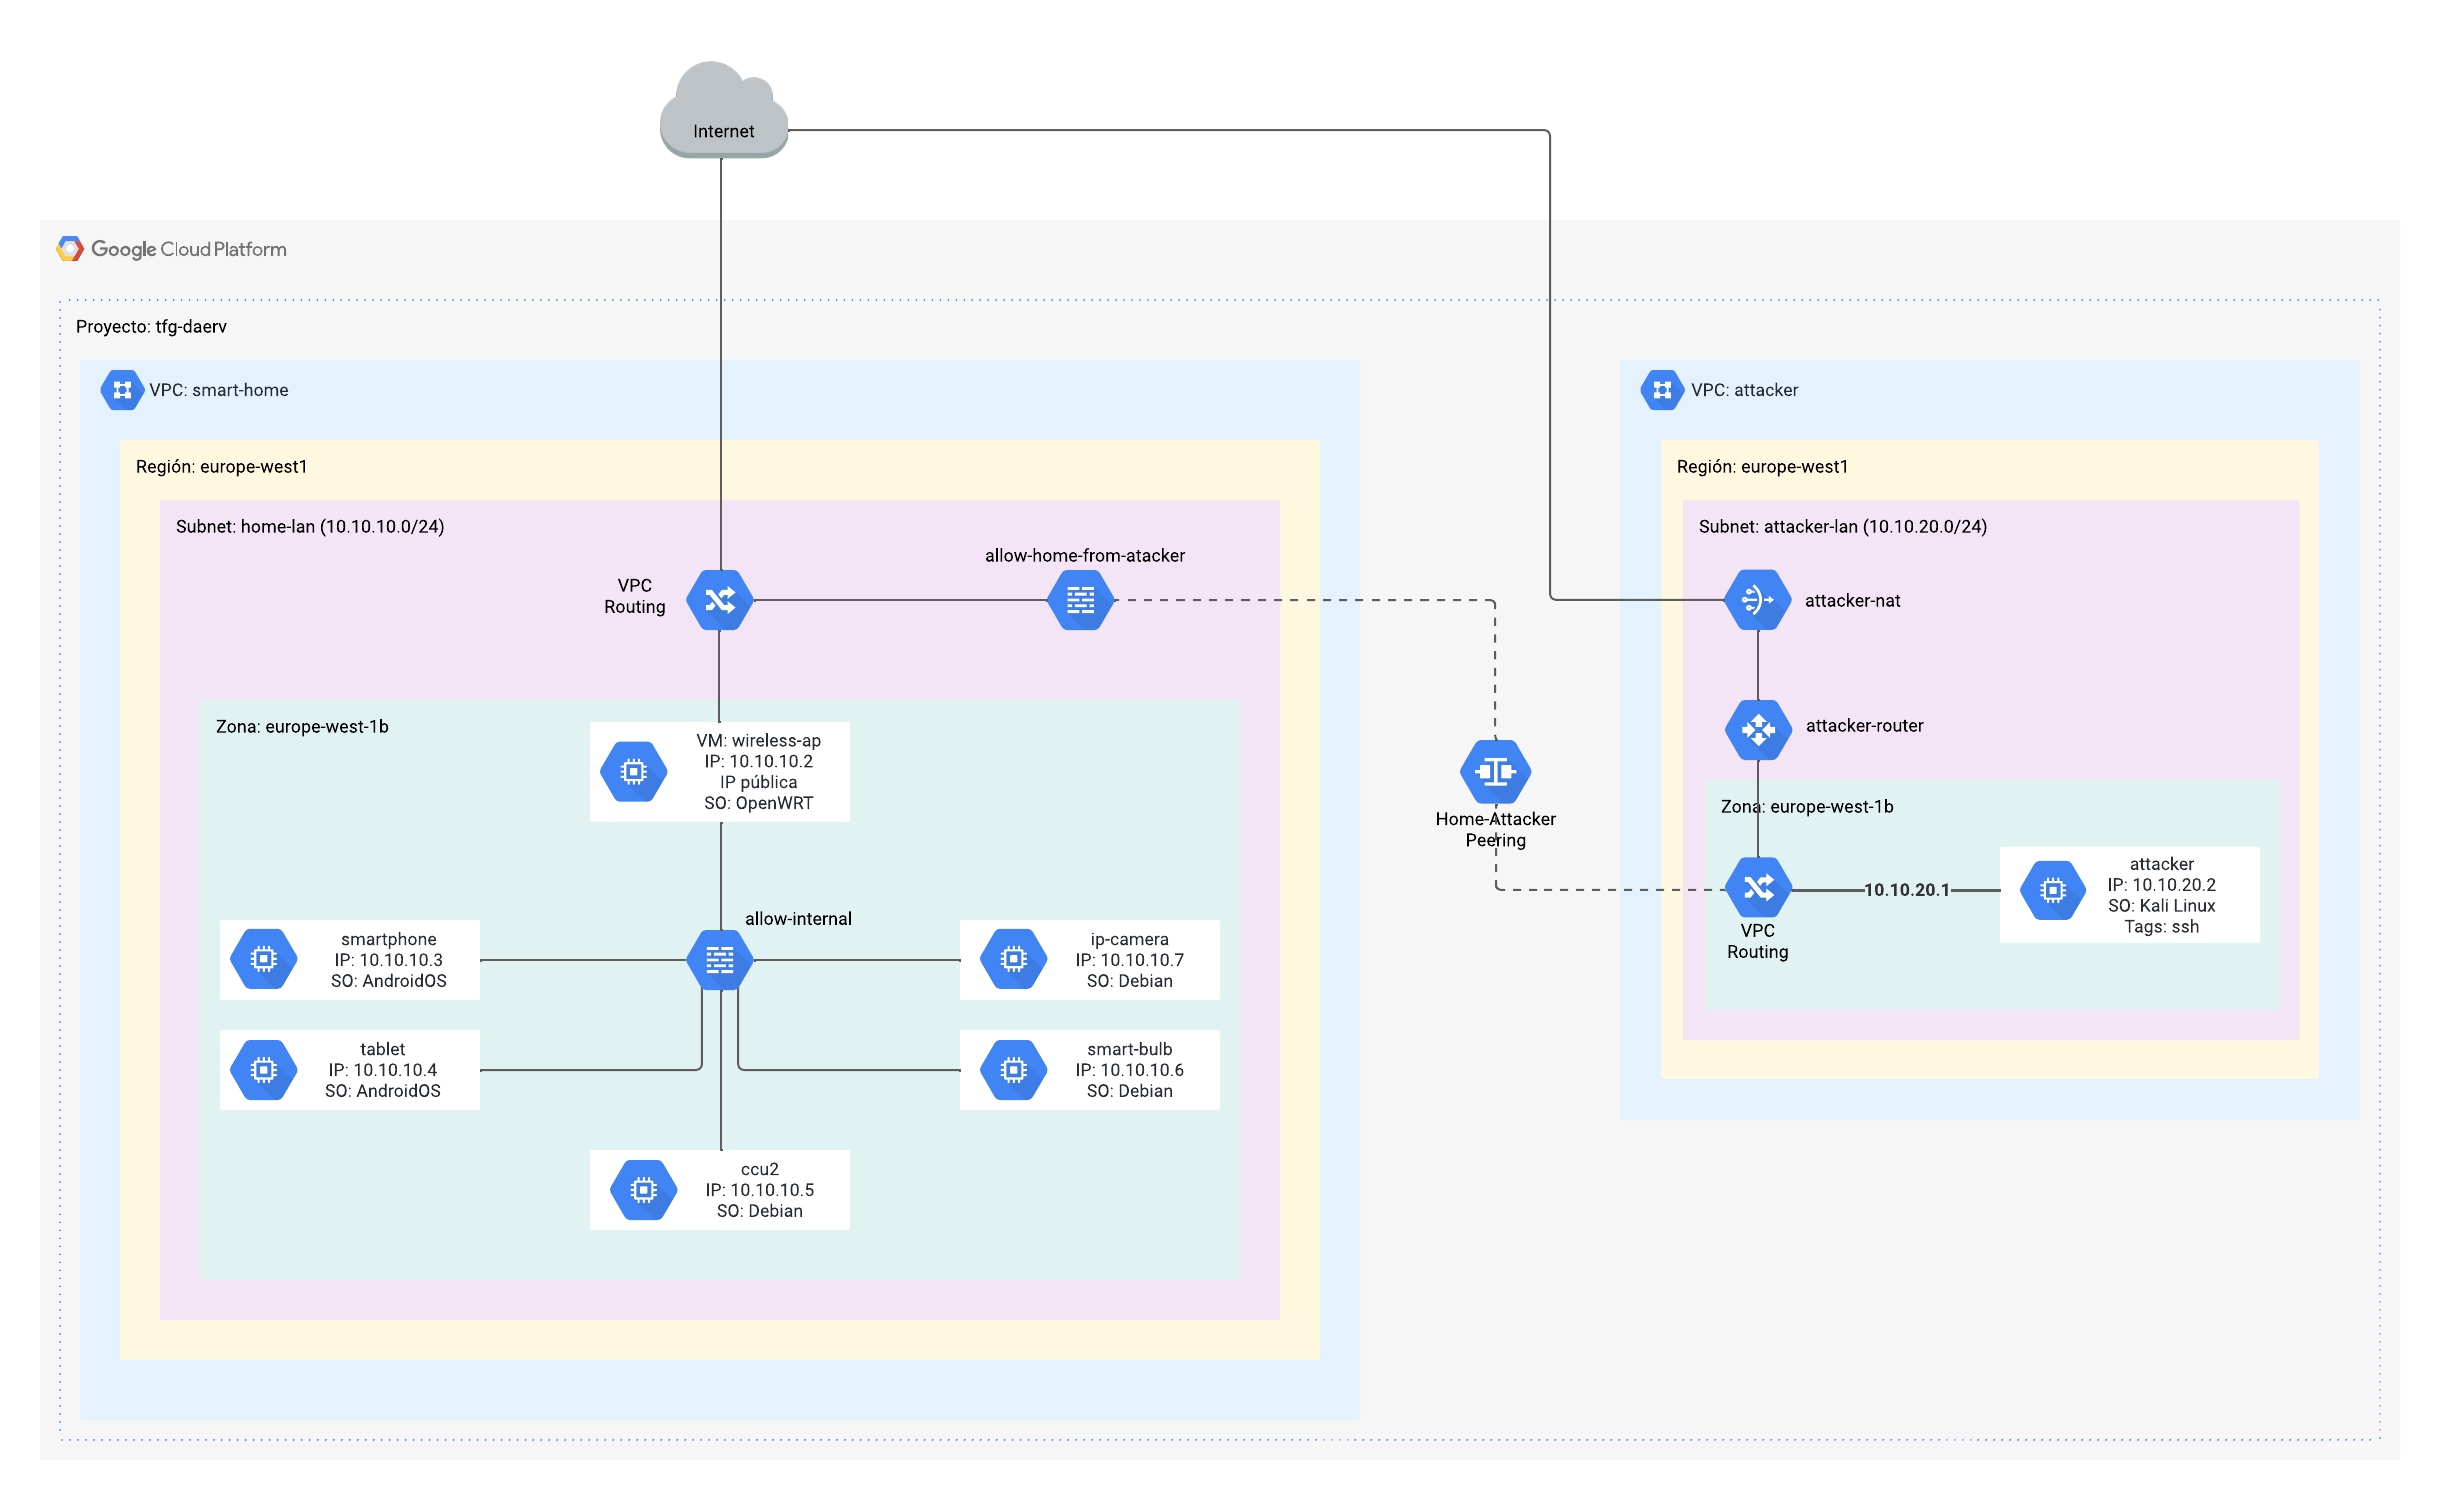
\includegraphics[width=1.45\textwidth, angle=270]{../imgs/desarrollo/escenarios-de-red/smart-home/EscenarioSmartHome.png}
  \caption{Implementación en GCP del escenario Smart Home}
  \label{fig:sh-i}
  \end{figure}
  \clearpage

\subsection{SCADA} \label{sec:sh}
\subsubsection{Descripción}

  \begin{figure}[h]
  \centering
  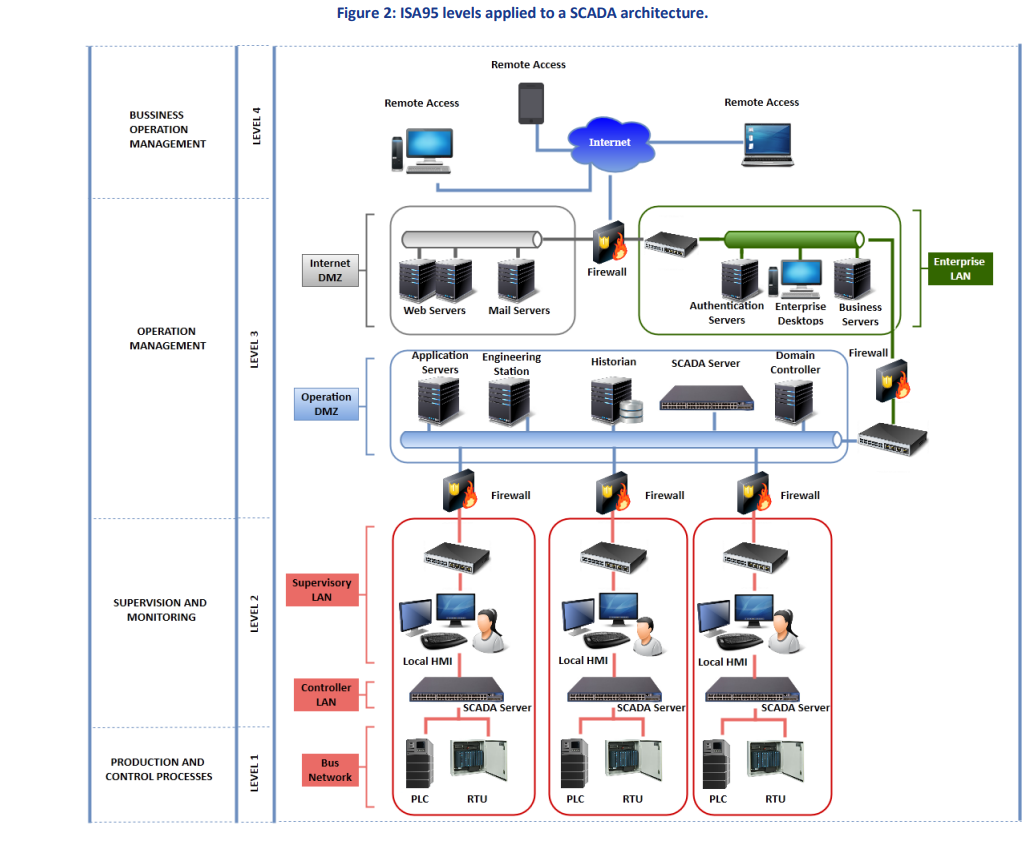
\includegraphics[width=0.9\textwidth]{../imgs/desarrollo/escenarios-de-red/SCADA/SCADA_Network_2.PNG}
  \caption{Topología del escenario SCADA}
  \label{fig:scada-t}
  \end{figure}

  \clearpage
\subsubsection{Implementación}
  El escenario SCADA consta de una única VPC, en la que se pueden diferenciar dos grandes partes, la parte superior sería la parte IT (corporativa) y la inferior la parte OT (operativa). La VPC está segmentada en varias subredes: \textit{internet-dmz}, \textit{enterprise-lan}, y \textit{operation-dmz} forman la parte correspondiente a la parte IT y \text-it{ot-lan} simula la parte OT. 

  \begin{table}[h]
    \begin{center}
      \begin{tabular}{ | m{1cm} | w{c}{3cm} | w{c}{2,5cm} | m{7,5cm} | }
        \hline\rowcolor{oranget} \centering\textbf{VPC} & \textbf{LAN} & \textbf{Rango IP} & \textbf{Equipos} \\ \hline
        \multirow{4}{*}{scada} & internet-dmz & 10.10.10.0/24 & web-server, mail-server \\ \cline{2-4}
         & enterprise-lan & 10.10.20.0/24 & auth-server, business-server, enterprise-desktop \\ \cline{2-4}
         & operation-dmz & 10.10.30.0/24 & app-server, engineering-station, historian, scada-server, domain-controller \\ \cline{2-4}
         & ot-lan & 10.10.40.0/24 & local-hmi-pro, scada-server-pro, plc-pro, rtu-pro, local-hmi-pre, scada-server-pre, plc-pre, rtu-pre \\ \hline
        \end{tabular}
      \caption{Estructura del escenario SCADA}
      \label{tab:vpc4}
    \end{center}
  \end{table}

  El tráfico entre todas las LAN de la VPC está limitado por reglas de FW. Además, dentro de la subred OT se distingue una red de producción y otra de preproducción, que no deben tener conexión entre sí. Para ello, dentro de estas, se han definido reglas de FW de forma que cada dispositivo solo se pueda comunicar con los de su nivel inmediatamente superior o inferior. Es decir, mientras que en las LAN de IT la comunicación entre los dispositivos que la componen es amplia, en la parte OT esta comunicación está mucho más restringida.

  En cuanto al aprovisionamiento, se emplea el fichero \texttt{docker-provisioning.tftpl}. Este fichero tiene un funcionamiento igual al descrito en el escenario Smart Home, pero sin proxy, ya que esta VPC cuenta con Cloud Nat para proporcionar acceso a Internet a las instancias con dirección IP privada. Este script accede al contenido del fichero \texttt{os-release}, ubicado en el directorio \texttt{/etc/}, para determinar si el SO es Debian, Ubuntu, Centos o Fedora, instala Docker en función de dicho SO y arranca el contenedor deseado. Para arrancar el contenedor, a la hora de invocar al script se le pasan como argumentos la imagen Docker de la cual se quiere arrancar un contenedor, el tag (versión) de dicha imagen y argumentos opcionales como mapeo de puertos o un punto de entrada al contenedor.

  Se detallan a continuación las reglas de firewall. Los servidores de correo y mail son públicos. Por eso las reglas \textit{allow-web} y \textit{allow-mail} permiten conexiones a estos desde cualquier dirección IP a través de los puertos correspondientes, que en el caso del servidor web son el 80 y el 443 (http y https) y en el caso del servidor de correo el 465 y 587 (SMTP). El puerto 25, típico de SMTP, no se ha incluido ya que Google Cloud bloquea siempre las conexiones a este debido al riesgo de abuso. El resto de reglas hacen posible la conexión privada entre las tres subredes IT, la conexión entre la subred de operaciones y los hmi, la conexión entre cada hmi y su servidor SCADA y, finalmente, la comunicación interna entre el servidor SCADA, el PLC y el RTU. Nótese que se ha obviado la columna correspondiente a la VPC donde aplica la regla ya que sólo hay una VPC.

   \begin{table}[h]
    \begin{center}
      \footnotesize\begin{tabular}{ | m{2cm} | w{c}{1,5cm} | m{2cm} | m{2cm} | m{2cm} | w{c}{1,25cm} | w{c}{1,25cm} | }
        \hline\rowcolor{oranget} \centering\textbf{Nombre} & \textbf{Dirección} & \centering\textbf{Origen} & \centering\textbf{Destino} & \centering\textbf{Protocolos} & \textbf{Puertos} & \textbf{Acción} \\ \hline
        allow-web & INGRESS & 0.0.0.0/0 & web-server (tag) & \centering TCP & 80, 443 & ALLOW  \\ \hline\rowcolor{oranger}
        allow-mail & INGRESS & 0.0.0.0/0 & mail-server (tag) & \centering TCP & 465, 587 & ALLOW  \\ \hline
        allow-enterprise & INGRESS & 10.10.10.0/24 10.10.20.0/24 10.10.30.0/24 & enterprise (tag) & TCP, UDP, ICMP & 0-65535 & ALLOW \\ \hline\rowcolor{oranger}
        allow-operation & INGRESS & 10.10.10.0/24 10.10.20.0/24 10.10.30.0/24 & operation (tag) & TCP, UDP, ICMP & 0-65535 & ALLOW \\ \hline
        allow-ops-from-hmi & INGRESS & hmi-pro (tag) hmi-pre (tag) & operation (tag) & TCP, UDP, ICMP & 0-65535 & ALLOW \\ \hline\rowcolor{oranger}
        allow-hmi-pro-from-ops & INGRESS & operation (tag) & hmi-pro (tag) & TCP, UDP, ICMP & 0-65535 & ALLOW \\ \hline
        allow-hmi-pre-from-ops & INGRESS & operation (tag) & hmi-pre (tag) & TCP, UDP, ICMP & 0-65535 & ALLOW \\ \hline\rowcolor{oranger}
        allow-hmi-server-pro & INGRESS & hmi-pro (tag) scada-pro (tag) & hmi-pro (tag) scada-pro (tag) & TCP, UDP, ICMP & 0-65535 & ALLOW \\ \hline 
        allow-hmi-server-pre & INGRESS & hmi-pre (tag) scada-pre (tag) & hmi-pre (tag) scada-pre (tag) & TCP, UDP, ICMP & 0-65535 & ALLOW \\ \hline\rowcolor{oranger}
        allow-bus-pro & INGRESS & scada-pro (tag) plc-pro (tag) rtu-pro (tag) & scada-pro (tag) plc-pro (tag) rtu-pro (tag) & TCP, UDP, ICMP & 0-65535 & ALLOW \\ \hline
        allow-bus-pre & INGRESS & scada-pre (tag) plc-pre (tag) rtu-pre (tag) & scada-pre (tag) plc-pre (tag) rtu-pre (tag) & TCP, UDP, ICMP & 0-65535 & ALLOW \\ \hline\rowcolor{oranger}

      \end{tabular}
      \caption{Reglas de FW del escenario SCADA}
      \label{tab:fw4}
    \end{center}
  \end{table}

  \clearpage
  \begin{figure}[h]
  \centering
  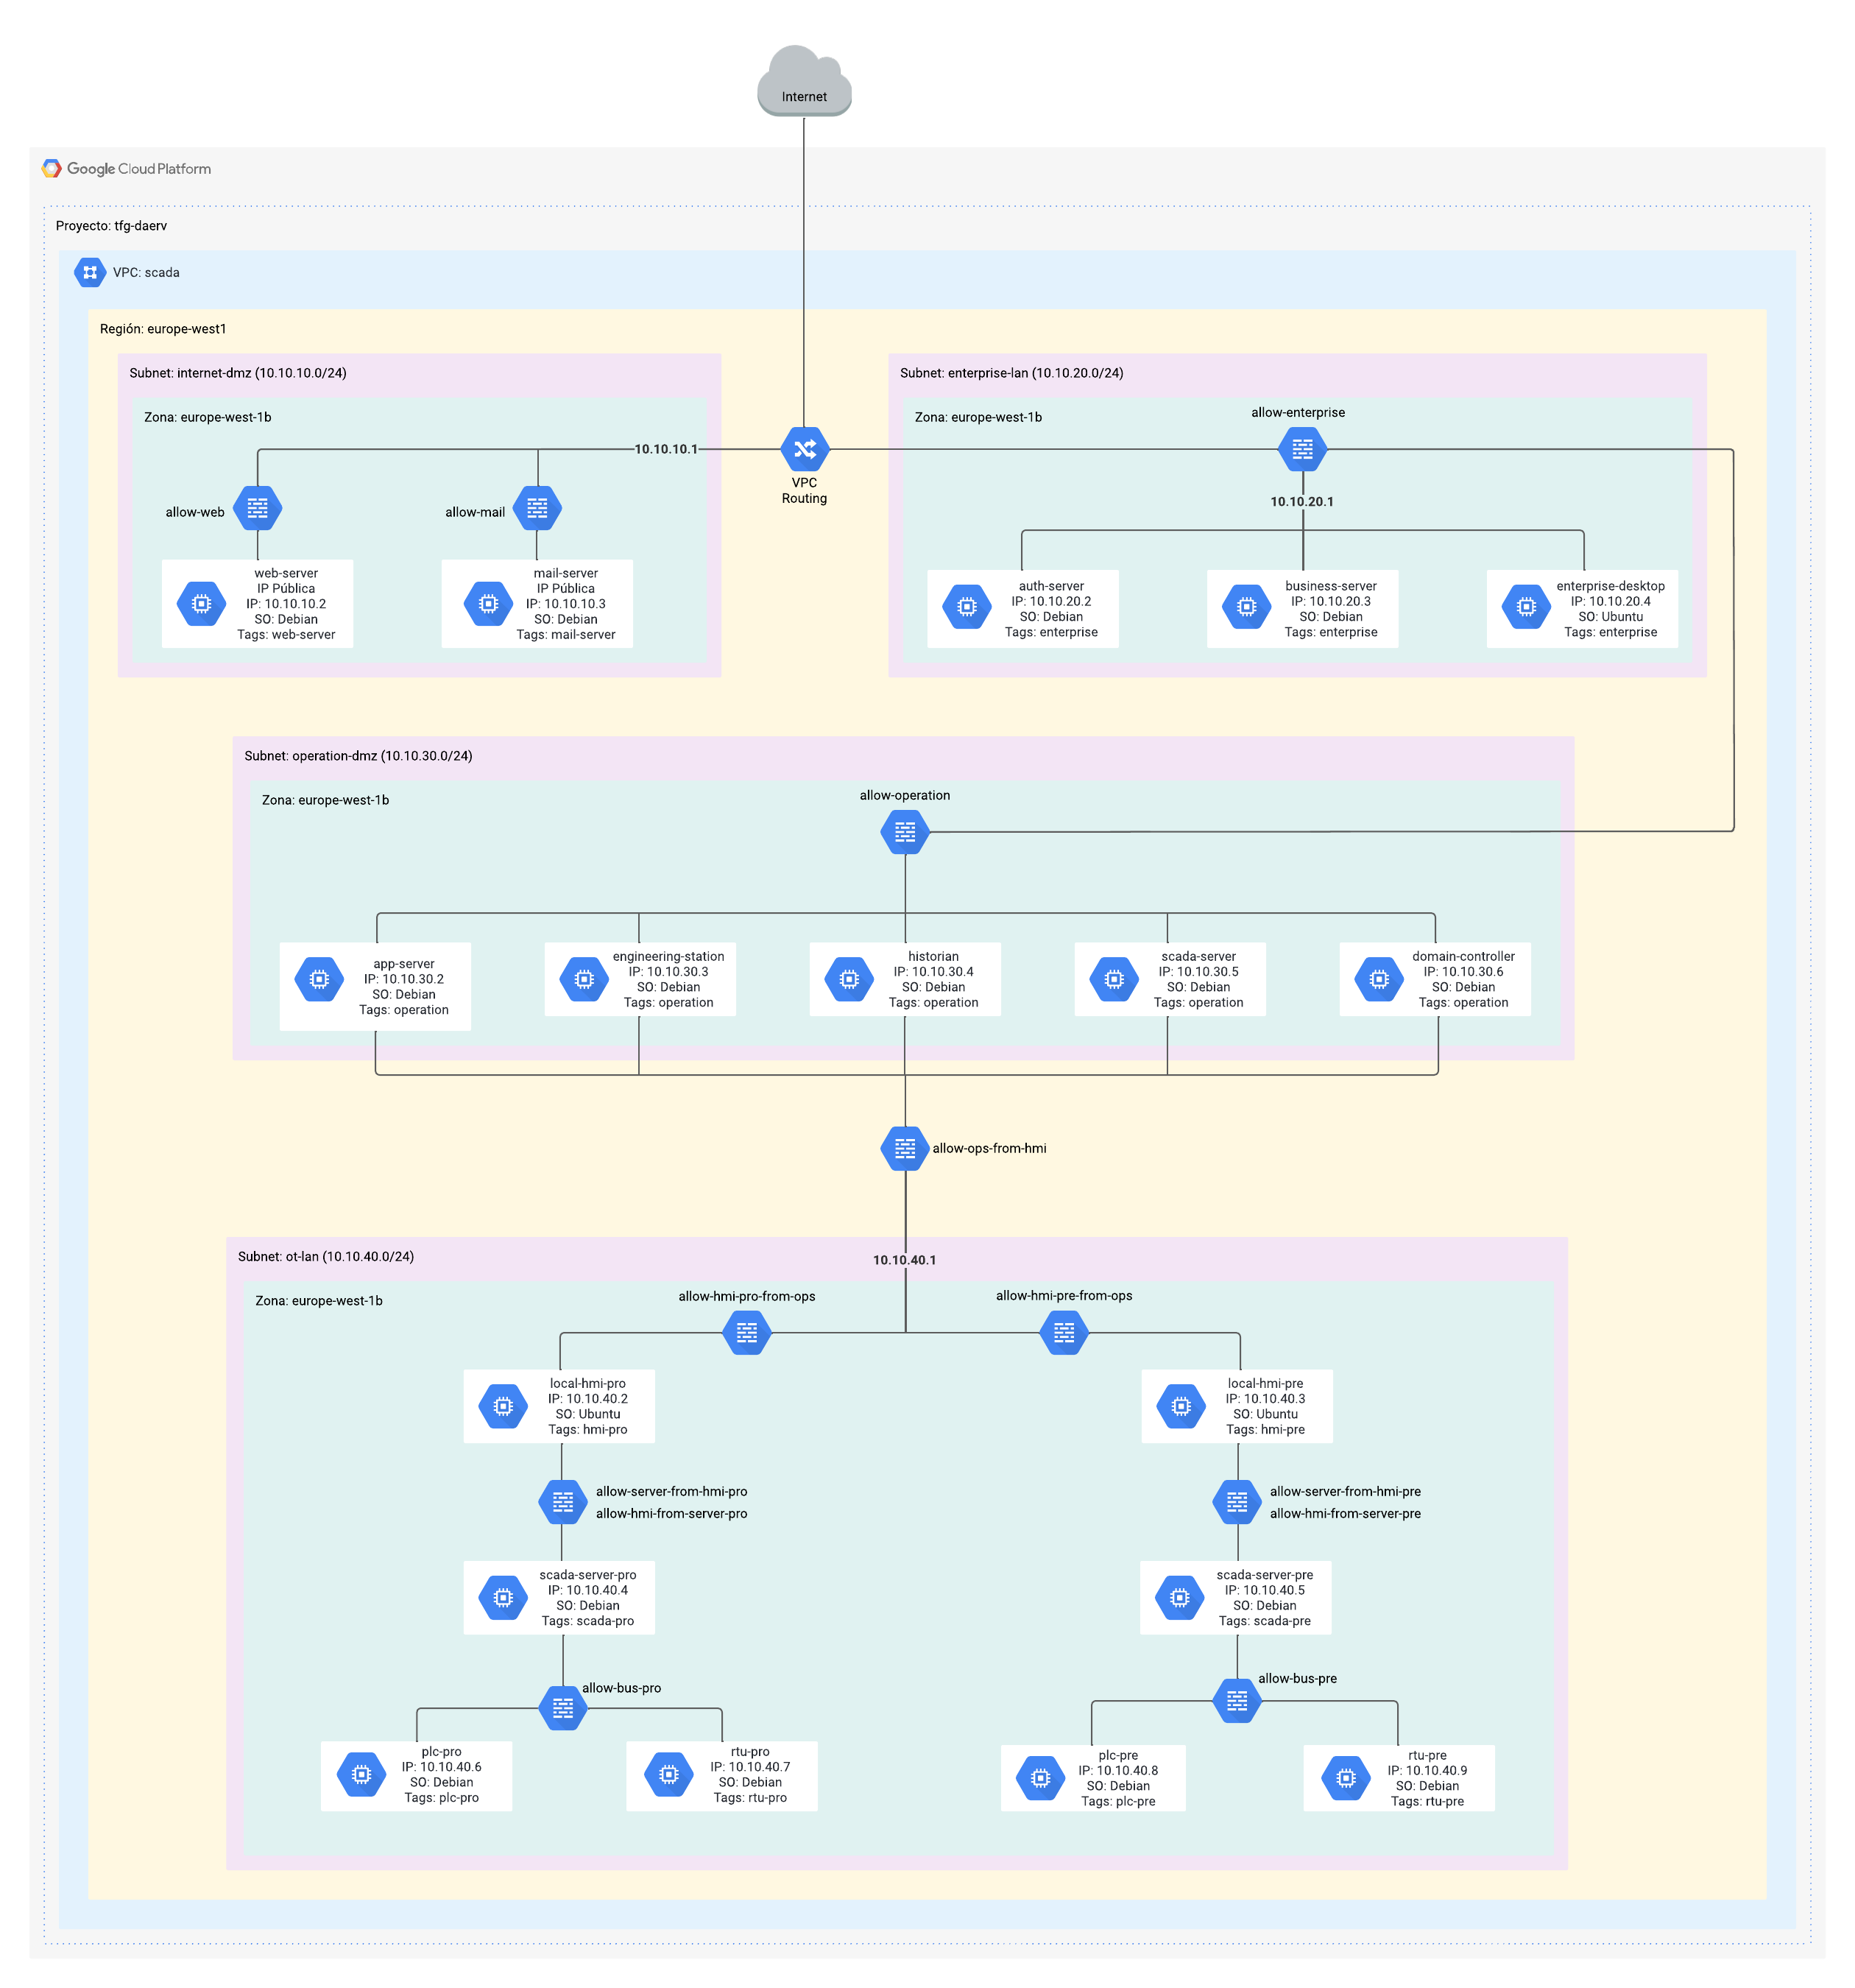
\includegraphics[width=\textwidth]{../imgs/desarrollo/escenarios-de-red/SCADA/EscenarioSCADA.png}
  \caption{Implementación en GCP del escenario SCADA}
  \label{fig:scada-i}
  \end{figure}
  \clearpage
